\documentclass[12pt,a4paper]{report}

% ---------- packages (all available in texlive basic) ----------
\usepackage[utf8]{inputenc}
\usepackage[T1]{fontenc}
\usepackage[margin=2.5cm]{geometry}
\usepackage{hyperref}
\usepackage{booktabs}
\usepackage{longtable}
\usepackage{tabularx}
\usepackage{array}
\usepackage{listings}
\usepackage{xcolor}
\usepackage{graphicx}
\usepackage{float}
\usepackage{amsmath}

% ---------- paragraph spacing (replaces parskip package) ----------
\setlength{\parskip}{6pt}
\setlength{\parindent}{0pt}

% ---------- line breaking (prevents text overflowing margins) ----------
\emergencystretch=3em
\tolerance=1500
\hbadness=1500

% ---------- hyperref setup ----------
\hypersetup{
    colorlinks=true,
    linkcolor=blue!60!black,
    urlcolor=blue!70!black,
    citecolor=green!50!black,
    pdftitle={Part 2 - Architecture Report: Omnichannel Commerce Core},
    pdfauthor={Maria Linhares, Rui Machado, Guilherme Rosa, Gabriel Silva},
}

% ---------- code listings ----------
\lstset{
    basicstyle=\ttfamily\small,
    keywordstyle=\color{blue!70!black}\bfseries,
    commentstyle=\color{gray}\itshape,
    stringstyle=\color{orange!80!black},
    backgroundcolor=\color{gray!8},
    frame=single,
    rulecolor=\color{gray!40},
    breaklines=true,
    breakatwhitespace=true,
    numbers=left,
    numberstyle=\tiny\color{gray},
    xleftmargin=1.5em,
    framexleftmargin=1.5em,
    tabsize=4,
    showstringspaces=false,
}

% ---------- simple coloured boxes (no tcolorbox needed) ----------
% Uses savebox to collect block content before passing it to \colorbox,
% which avoids the "Not allowed in LR mode" error when itemize/description
% are used inside the boxes.

\newsavebox{\decisionboxbuf}
\newenvironment{decisionbox}{%
    \vspace{0.5em}\par
    \begin{lrbox}{\decisionboxbuf}%
    \begin{minipage}{\dimexpr\linewidth-2\fboxsep}%
    \vspace{0.4em}\par\textbf{Decision}\par\smallskip}{%
    \par\vspace{0.4em}%
    \end{minipage}%
    \end{lrbox}%
    \noindent\colorbox{blue!8}{\usebox{\decisionboxbuf}}%
    \vspace{0.5em}\par}

\newsavebox{\riskboxbuf}
\newenvironment{riskbox}{%
    \vspace{0.5em}\par
    \begin{lrbox}{\riskboxbuf}%
    \begin{minipage}{\dimexpr\linewidth-2\fboxsep}%
    \vspace{0.4em}\par}{%
    \par\vspace{0.4em}%
    \end{minipage}%
    \end{lrbox}%
    \noindent\colorbox{orange!12}{\usebox{\riskboxbuf}}%
    \vspace{0.5em}\par}

\newsavebox{\scopeboxbuf}
\newenvironment{scopebox}{%
    \vspace{0.5em}\par
    \begin{lrbox}{\scopeboxbuf}%
    \begin{minipage}{\dimexpr\linewidth-2\fboxsep}%
    \vspace{0.4em}\par}{%
    \par\vspace{0.4em}%
    \end{minipage}%
    \end{lrbox}%
    \noindent\colorbox{gray!10}{\usebox{\scopeboxbuf}}%
    \vspace{0.5em}\par}

% ---------- column types ----------
\newcolumntype{L}[1]{>{\raggedright\arraybackslash}p{#1}}
\newcolumntype{C}[1]{>{\centering\arraybackslash}p{#1}}

% ==========================================================
\begin{document}

% ---------- title page ----------
\begin{titlepage}
    \centering
    \vspace*{2cm}
    {\scshape\LARGE Software Architecture \par}
    \vspace{0.5cm}
    {\scshape\large Assignment 2, Part 2 \par}
    \vspace{1.5cm}
    {\Huge\bfseries Omnichannel Commerce Core\\[0.4em]
    \Large Architecture Report \par}
    \vspace{0.5cm}
    {\large\itshape Scenario C: nopCommerce Architectural Evolution \par}
    \vspace{2cm}
    \rule{\textwidth}{0.5pt}
    \vspace{0.5cm}
    {\large
    Guilherme Rosa\\
    Rui Machado\\
    Maria Linhares\\
    Gabriel Silva \par}
    \vspace{0.5cm}
    \rule{\textwidth}{0.5pt}
    \vspace{1.5cm}
    {\large May 2026 \par}
    \vfill
    {\small Deadline: 02-03 June 2026}
\end{titlepage}

% ---------- table of contents ----------
\tableofcontents
\listoffigures
\listoftables
\newpage

% ---------- chapters ----------
\chapter{Introduction}
\label{ch:introduction}

\section{Context and Scenario}

This report documents the Part~2 implementation of Scenario~C, \textit{Omnichannel Commerce Core}, for the Software Architecture assignment. The system under evolution is \textbf{nopCommerce}, an open-source e-commerce platform, extended to coordinate reliably with external operational systems: an OpenBoxes warehouse management system (WMS), a WireMock-simulated carrier, and a RabbitMQ message broker.

The domain is modelled for \textbf{VerdeMart Retail}, a fictional retailer operating both online and physical channels.

The team is composed of Maria Linhares, Rui Machado, Guilherme Rosa, and Gabriel Silva.

\section{The Architectural Bet}

The central decision of Part~1, carried into implementation in Part~2, is stated in one sentence:

\begin{decisionbox}
Replace the synchronous stock decrement inside \texttt{OrderProcessingService} with an outbox-published event, so order acceptance survives warehouse degradation and reconciles on recovery.
\end{decisionbox}

This single change, and everything it pulls along, is the assignment. It directly addresses \textbf{QA-1} (availability under warehouse degradation) and sets the foundation for \textbf{QA-2} (stock consistency) and \textbf{QA-3} (order placement throughput).

\section{Report Structure}

\begin{description}
    \item[Chapter~\ref{ch:evolution}] Architecture evolution from Part~1 plan to actual implementation: what changed and why.
    \item[Chapter~\ref{ch:implementation}] Implementation overview of both plugins built inside the nopCommerce monolith.
    \item[Chapter~\ref{ch:adr}] Architecture Decision Records: updated from Part~1 and new decisions made during implementation.
    \item[Chapter~\ref{ch:crosscutting}] Cross-cutting concerns: idempotency, error handling, observability, security.
    \item[Chapter~\ref{ch:traceability}] Traceability matrix linking business drivers to QA scenarios to implementation.
    \item[Chapter~\ref{ch:demo}] Demo orchestration: the four scenarios and their success criteria.
    \item[Chapter~\ref{ch:tradeoffs}] Defence of tradeoffs, scope cuts, and known limitations.
\end{description}

\chapter{Architecture Evolution}
\label{ch:evolution}

This chapter describes how the target architecture defined in Part~1 evolved during implementation. It covers what remained unchanged, what was refined, and what was cut.

\section{What Remained Unchanged}

The five bounded contexts identified in Part~1 held through implementation without revision:

\begin{enumerate}
    \item \textbf{Catalog:} inside nopCommerce; owns product definitions, pricing, categories.
    \item \textbf{Order Management:} inside nopCommerce; owns the order lifecycle, customer intent, payment authorisation.
    \item \textbf{Identity:} inside nopCommerce (cross-cutting); owns customer accounts and authentication.
    \item \textbf{Inventory / Warehouse:} extracted; owns authoritative stock truth, reservations, stock movements.
    \item \textbf{Shipping / Fulfillment:} extracted; owns carrier dispatch, tracking, delivery state.
\end{enumerate}

The \textbf{transactional outbox} as the reliability mechanism was also confirmed and not revisited. The feasibility spike (Part~1, \S7) had already de-risked the critical constraint: \texttt{PlaceOrderAsync} does not run inside an ambient \texttt{TransactionScope}, so the outbox decorator must supply one.

\section{Structural Change: Two Plugins Instead of One}

Part~1 described a single plugin (\texttt{Nop.Plugin.Misc.OmnichannelOutbox}) carrying both the outbox write and the inbound RabbitMQ subscriber. During implementation, the inbound side was split into a \textbf{separate plugin}: \texttt{Nop.Plugin.Misc.OmnichannelConsumers}.

\begin{table}[H]
\centering
\caption{Plugin split rationale}
\label{tab:plugin-split}
\begin{tabularx}{\textwidth}{@{} L{4.5cm} X @{}}
\toprule
\textbf{Plugin} & \textbf{Responsibility} \\
\midrule
\texttt{OmnichannelOutbox} & Outbox write path: entity, publisher decorator, dispatcher, RabbitMQ publisher, TransactionScope decorator, retention cleanup \\
\addlinespace
\texttt{OmnichannelConsumers} & Inbound path: RabbitMQ subscriber, inbox deduplication, event handlers, compensation orchestration \\
\bottomrule
\end{tabularx}
\end{table}

This separation follows the single-responsibility principle at plugin granularity and mirrors the Part~1 ADD iteration structure (Iteration~1 = outbox, Iteration~2 = consumers and stock projection).

\section{New: \texttt{Compensated} Order State}

The \texttt{Compensated} state was added to the \texttt{OrderStatus} enum in \texttt{Nop.Core}. This was anticipated in Part~1 but is now concrete code. The state is reached when the Inventory service rejects a stock reservation and the compensation flow (payment release, customer notification) completes.

\begin{figure}[H]
\centering
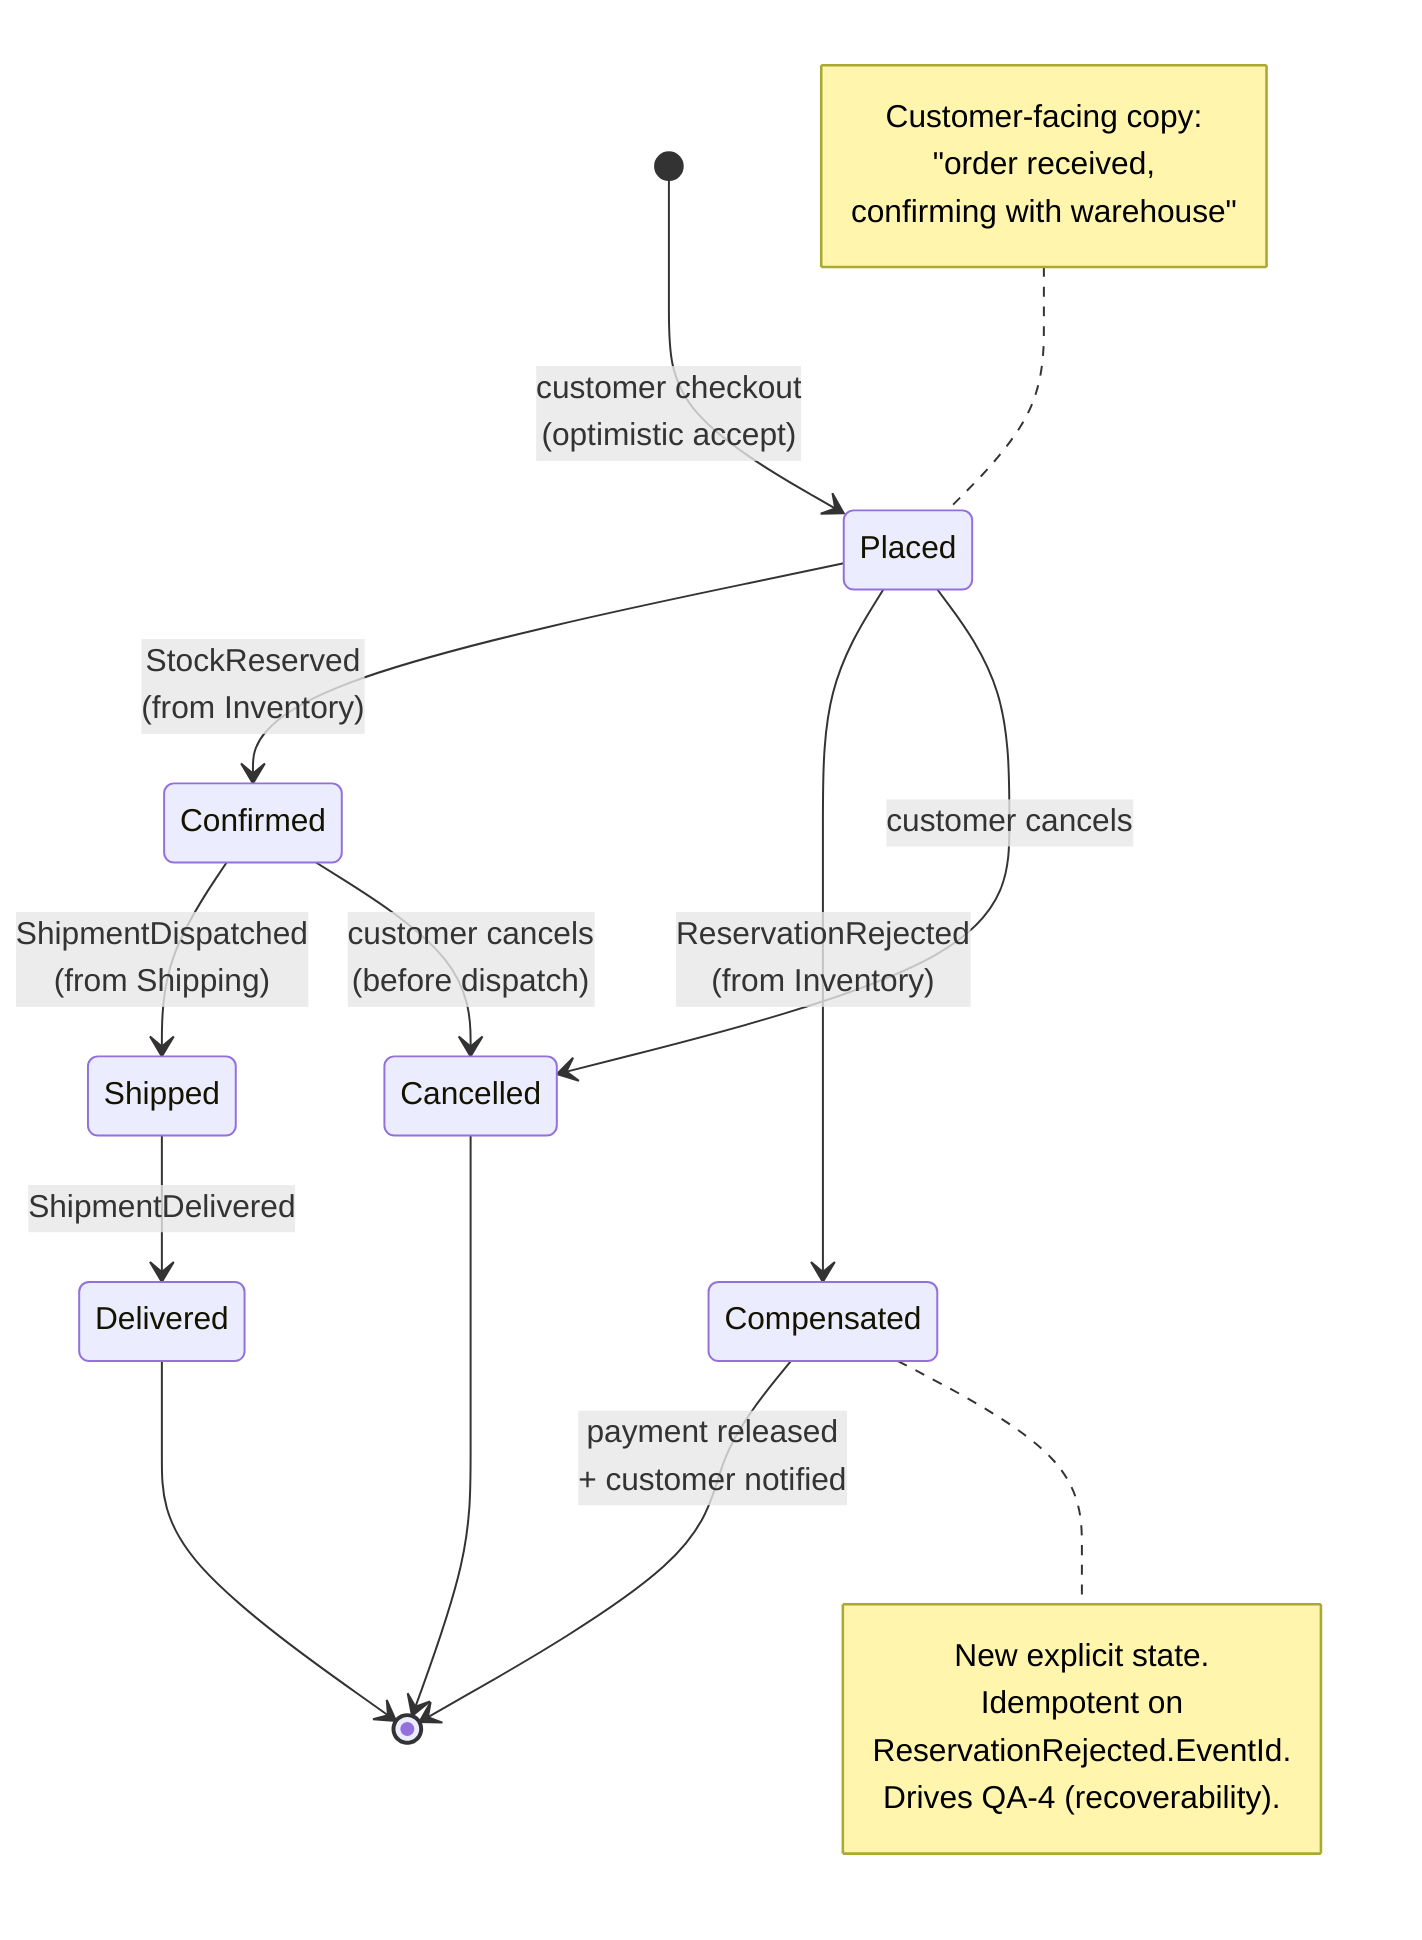
\includegraphics[width=\textwidth]{figures/order-lifecycle.png}
\caption{Order lifecycle state machine including the new \texttt{Compensated} state}
\label{fig:order-lifecycle}
\end{figure}

\section{New: Inbox Deduplication}

Part~1 stated that consumers must be idempotent but left the mechanism open. The implementation chose an \textbf{inbox table} approach: a \texttt{ProcessedInboxMessage} entity records every \texttt{EventId} that has been handled. Before processing any inbound message, \texttt{InboxDeduplicationService} checks for an existing record. Duplicates are silently discarded.

This satisfies the at-least-once delivery guarantee without requiring exactly-once semantics from RabbitMQ.

\section{Event Contracts Settled}

The event contracts were implemented as dedicated event classes in \texttt{Nop.Core.Domain}:

\begin{table}[H]
\centering
\caption{Cross-context event contracts}
\label{tab:events}
\begin{tabularx}{\textwidth}{@{} L{5cm} L{2.5cm} X @{}}
\toprule
\textbf{Event} & \textbf{Direction} & \textbf{Published when} \\
\midrule
\texttt{OrderPlacedEvent} & Outbound & Customer places an order \\
\texttt{StockReservedEvent} & Inbound & Inventory confirms stock reservation \\
\texttt{Reservation\-Rejected\-Event} & Inbound & Inventory cannot fulfil the reservation \\
\texttt{OrderConfirmedEvent} & Outbound & Order moves to \texttt{Confirmed} state \\
\texttt{StockLevelChangedEvent} & Inbound & External stock movement \\
\texttt{ShipmentDispatchedEvent} & Inbound & Shipping service dispatches the parcel \\
\texttt{OrderCompensatedEvent} & Internal & Compensation flow completes \\
\bottomrule
\end{tabularx}
\end{table}

\section{Scope Cuts Carried Over From Part~1}

All acknowledged scope cuts from Part~1 remain in force:

\begin{scopebox}
\begin{itemize}
    \item Identity stays as-is (no federated SSO across channels).
    \item Payment is folded into Order Management, with no separate Payment service.
    \item Shipping equals Fulfillment: one extracted service, not two.
    \item Single nopCommerce instance: no Redis, no horizontal scaling.
    \item The outbox lives \textbf{inside the monolith process} as an \texttt{IScheduleTask}, not as a separate worker.
\end{itemize}
\end{scopebox}

\chapter{Implementation Overview}
\label{ch:implementation}

\section{OmnichannelOutbox Plugin}

\texttt{Nop.\-Plugin.\-Misc.\-Omnichannel\-Outbox} is the outbox write path. It is registered via \texttt{INopStartup} and requires no changes to nopCommerce core.

\subsection{OutboxMessage Entity}

\texttt{OutboxMessage} is persisted to a dedicated table created by a FluentMigrator schema migration shipped with the plugin. Key fields:

\begin{table}[H]
\centering
\caption{\texttt{OutboxMessage} schema}
\label{tab:outbox-schema}
\begin{tabularx}{\textwidth}{@{} L{4cm} L{2.5cm} X @{}}
\toprule
\textbf{Column} & \textbf{Type} & \textbf{Purpose} \\
\midrule
\texttt{Id} & \texttt{int} & Primary key \\
\texttt{EventId} & \texttt{Guid} & Idempotency key for consumers \\
\texttt{MessageType} & \texttt{string} & Fully qualified event type name \\
\texttt{Payload} & \texttt{string} & JSON-serialised event payload \\
\texttt{OccurredOnUtc} & \texttt{DateTime} & When the event was written \\
\texttt{DispatchedOnUtc} & \texttt{DateTime?} & Null until the dispatcher confirms broker ack \\
\texttt{Attempts} & \texttt{int} & Incremented on each failed dispatch attempt \\
\bottomrule
\end{tabularx}
\end{table}

\subsection{OutboxEventPublisherDecorator}

Wraps nopCommerce's \texttt{IEventPublisher}. For a \textbf{whitelisted set} of cross-context event types, it writes an \texttt{OutboxMessage} row instead of (or in addition to) calling in-process consumers. All other event types pass through unchanged, preserving compatibility with existing plugins (Brevo, Omnisend, etc.).

The whitelist is the explicit seam between bounded contexts. Adding a new cross-context event requires editing the whitelist — deliberate friction to prevent accidental coupling.

\subsection{OrderProcessingServiceDecorator}

Wraps \texttt{IOrderProcessingService} to supply the missing \texttt{TransactionScope} around the order-creation path. The decorator uses:

\begin{lstlisting}[language={[Sharp]C}, caption={TransactionScope pattern used in the decorator}]
using var scope = new TransactionScope(
    TransactionScopeOption.Required,
    new TransactionOptions { IsolationLevel = IsolationLevel.ReadCommitted },
    TransactionScopeAsyncFlowOption.Enabled);

var result = await _inner.PlaceOrderAsync(processPaymentRequest);

if (result.Success)
    scope.Complete();
\end{lstlisting}

Two non-obvious constraints confirmed by the feasibility spike:
\begin{itemize}
    \item \texttt{Transaction\-Scope\-Async\-Flow\-Option.\-Enabled} is mandatory: without it, \texttt{Transaction.\-Current} does not flow across the first \texttt{await} and the outbox row falls outside the transaction.
    \item Isolation level is tuned to \texttt{ReadCommitted} to avoid a hidden throughput tax from the default \texttt{Serializable} (QA-3 concern).
\end{itemize}

\subsection{OutboxDispatcherTask}

An \texttt{IScheduleTask} polling the outbox table on a 5-10~s cadence. For each undispatched row it publishes to RabbitMQ via \texttt{RabbitMqPublisher} and, on broker ack, sets \texttt{DispatchedOnUtc}. On failure it increments \texttt{Attempts}; rows exceeding a configured maximum remain in the table as a dead-letter view for manual inspection.

\subsection{OutboxRetentionTask}

A second \texttt{IScheduleTask} that deletes dispatched outbox rows older than 7~days, preventing unbounded table growth (Risk~R5 mitigation).

% -------------------------------------------------------
\section{OmnichannelConsumers Plugin}

\texttt{Nop.\-Plugin.\-Misc.\-Omnichannel\-Consumers} is the inbound path. It subscribes to RabbitMQ, deduplicates messages, and routes them to the appropriate handler.

\subsection{RabbitMqSubscriberTask}

An \texttt{IScheduleTask} that drives the RabbitMQ consumer loop. On each tick it drains available messages from the configured queues and dispatches them to \texttt{IInboxMessageHandler} implementations.

\subsection{InboxDeduplicationService}

Before any handler runs, \texttt{InboxDeduplicationService} checks whether the message's \texttt{EventId} already exists in the \texttt{ProcessedInboxMessage} table. If it does, the message is silently discarded. This enforces idempotency at the infrastructure layer, freeing individual handlers from duplicating the check.

\texttt{ProcessedInboxMessage} is persisted via a dedicated schema migration in this plugin.

\subsection{Event Handlers}

\begin{table}[H]
\centering
\caption{Inbound event handlers}
\label{tab:handlers}
\small
\begin{tabularx}{\textwidth}{@{} L{5.5cm} X @{}}
\toprule
\textbf{Handler} & \textbf{Behaviour} \\
\midrule
\texttt{Stock\-Reserved\-Handler} & Moves the order from \texttt{Placed} to \texttt{Confirmed}; publishes \texttt{Order\-Confirmed\-Event} to the outbox for the Shipping service \\
\addlinespace
\texttt{Reservation\-Rejected\-Handler} & Delegates to \texttt{Compensation\-Service}: voids the payment, notifies the customer, transitions order to \texttt{Compensated} \\
\addlinespace
\texttt{Stock\-Level\-Changed\-Handler} & Updates the Catalog stock projection (read model) inside the monolith \\
\addlinespace
\texttt{Shipment\-Dispatched\-Handler} & Advances the order to \texttt{Shipped} state and records the tracking reference \\
\bottomrule
\end{tabularx}
\end{table}

\subsection{CompensationService}

Orchestrates the compensation flow on reservation rejection:
\begin{enumerate}
    \item Void or refund the payment authorisation.
    \item Send a customer notification (via nopCommerce's existing messaging infrastructure).
    \item Transition the order status to \texttt{Compensated}.
    \item Publish \texttt{OrderCompensatedEvent} (in-process, for audit trail).
\end{enumerate}

% -------------------------------------------------------
\section{Feature Flag: Synchronous Fallback}

A feature flag controls whether the legacy synchronous stock decrement inside \texttt{OrderProcessingService} remains active. During the migration period this flag allows the team to run both paths side-by-side and validate the asynchronous path before fully cutting over. This is the migration strategy for risk R2.

\chapter{Architecture Decision Records}
\label{ch:adr}

This chapter presents the Architecture Decision Records (ADRs) for Part~2. ADRs 1 to 4 are carried over from Part~1 with implementation notes. ADRs 5 and 6 are new decisions made during implementation.

\section*{ADR-1: Transactional Outbox (carried over, status: Implemented)}
\addcontentsline{toc}{section}{ADR-1: Transactional Outbox}

\textbf{Status:} Accepted. Implemented in \texttt{OmnichannelOutbox} plugin.

\subsection*{Decision}
Write cross-context events to an \texttt{OutboxMessage} table inside the same DB transaction as the order, then dispatch to RabbitMQ asynchronously via a polling \texttt{IScheduleTask}.

\subsection*{Implementation notes}
The \texttt{TransactionScopeAsyncFlowOption.Enabled} constraint discovered in the feasibility spike was confirmed in production code. Isolation level was tuned to \texttt{ReadCommitted} as anticipated. No further divergence from the Part~1 decision.

\subsection*{Alternatives considered (Part~1)}
\begin{itemize}
    \item Direct RabbitMQ publish from \texttt{IConsumer<OrderPlacedEvent>}: REJECTED (dual-write risk).
    \item XA / two-phase commit: REJECTED (RabbitMQ not an XA resource; operational complexity).
    \item CDC / Debezium log mining: REJECTED (engine-specific; out of scope).
    \item Synchronous publish inside the order transaction: REJECTED (broker in critical path).
\end{itemize}

\section*{ADR-2: Optimistic Stock Reservation (carried over, status: Implemented)}
\addcontentsline{toc}{section}{ADR-2: Optimistic Stock Reservation}

\textbf{Status:} Accepted. Implemented via \texttt{OrderPlacedEvent} outbox path and \texttt{StockReservedHandler} / \texttt{ReservationRejectedHandler}.

\subsection*{Decision}
Accept orders optimistically without a synchronous stock check. The \texttt{OrderPlaced} event instructs the Inventory service to attempt a reservation. If the reservation fails, the compensation flow transitions the order to \texttt{Compensated}.

\subsection*{Implementation notes}
The \texttt{Compensated} state is now concrete in \texttt{OrderStatus}. The compensation flow is implemented in \texttt{CompensationService}. No divergence from the Part~1 decision.

\section*{ADR-3: WireMock Carrier Simulation (carried over, status: Implemented)}
\addcontentsline{toc}{section}{ADR-3: WireMock Carrier Simulation}

\textbf{Status:} Accepted. Implemented in the Shipping Service.

\subsection*{Decision}
Use WireMock to simulate the carrier API, avoiding a dependency on a live external service during development and the demo.

\section*{ADR-4: Selective Context Extraction (carried over, status: Implemented)}
\addcontentsline{toc}{section}{ADR-4: Selective Context Extraction}

\textbf{Status:} Accepted. Inventory and Shipping services extracted; Catalog, Order Management, and Identity remain in the monolith.

\subsection*{Decision}
Extract only the contexts whose failure modes are operationally distinct (Inventory, Shipping). Keep the remaining contexts inside the nopCommerce monolith to avoid unnecessary operational complexity for a demo-scale system.

\section*{ADR-5: Two Plugins Instead of One (new)}
\addcontentsline{toc}{section}{ADR-5: Two Plugins Instead of One}

\textbf{Status:} Accepted. Decided during Part~2 implementation.

\subsection*{Context}
Part~1 described a single \texttt{OmnichannelOutbox} plugin. During implementation the outbox write path and the inbound subscriber path grew in different directions, with distinct failure domains and lifecycle concerns.

\subsection*{Decision}
Split into two plugins: \texttt{OmnichannelOutbox} (write path) and \texttt{OmnichannelConsumers} (read/inbound path).

\subsection*{Rationale}
\begin{itemize}
    \item Each plugin has a single deployment and failure mode.
    \item The two paths can be enabled/disabled independently without affecting the other.
    \item Mirrors the ADD iteration structure: Iteration~1 = outbox write, Iteration~2 = consumers.
\end{itemize}

\subsection*{Alternatives considered}
\begin{itemize}
    \item \textbf{Single plugin:} REJECTED: one plugin holding both the dispatcher and the subscriber creates a large, hard-to-test unit with mixed failure domains.
    \item \textbf{Separate process for consumers:} REJECTED: out of scope; the monolith process is already hosting the outbox dispatcher as an \texttt{IScheduleTask}.
\end{itemize}

\section*{ADR-6: Inbox Table Deduplication (new)}
\addcontentsline{toc}{section}{ADR-6: Inbox Table Deduplication}

\textbf{Status:} Accepted. Implemented in \texttt{InboxDeduplicationService} and \texttt{ProcessedInboxMessage} entity.

\subsection*{Context}
RabbitMQ delivers at-least-once. Part~1 stated that consumers must be idempotent but left the mechanism open.

\subsection*{Decision}
Persist a \texttt{ProcessedInboxMessage} record (keyed on \texttt{EventId}) for every handled message. Check for this record before processing. Duplicates are discarded without executing handler logic.

\subsection*{Rationale}
\begin{itemize}
    \item Handler logic (state transitions, payment voids, notifications) is not naturally idempotent; centralising the check at the infrastructure layer removes the burden from individual handlers.
    \item The \texttt{ProcessedInboxMessage} table doubles as an audit log of processed messages.
    \item The same \texttt{InboxRetentionTask} pattern used by the outbox cleans up old records.
\end{itemize}

\subsection*{Alternatives considered}
\begin{itemize}
    \item \textbf{Handler-level idempotency:} REJECTED: each handler would need to query its own state to determine whether the action had already been taken (e.g., ``is this order already Confirmed?''). This is error-prone and forces domain logic to carry infrastructure concerns.
    \item \textbf{Exactly-once delivery via RabbitMQ quorum queues:} REJECTED: quorum queues reduce but do not eliminate duplicates; does not remove the need for consumer-side idempotency.
\end{itemize}

\chapter{Cross-Cutting Concerns}
\label{ch:crosscutting}

\section{Idempotency}

Idempotency is enforced at two levels:

\begin{enumerate}
    \item \textbf{Outbox side:} each \texttt{OutboxMessage} carries a unique \texttt{EventId} (a \texttt{Guid} generated at write time). Consumers use this field as their deduplication key.
    \item \textbf{Consumer side:} \texttt{InboxDeduplicationService} checks \texttt{ProcessedInboxMessage} before any handler executes. If the \texttt{EventId} has already been recorded, the message is discarded. This makes all handlers idempotent by construction, regardless of their internal logic.
\end{enumerate}

\section{Error Handling and Dead-Letter Strategy}

\begin{table}[H]
\centering
\caption{Error handling strategy by failure point}
\label{tab:error-handling}
\begin{tabularx}{\textwidth}{@{} L{3cm} L{4cm} X @{}}
\toprule
\textbf{Failure point} & \textbf{Behaviour} & \textbf{Operator action} \\
\midrule
Outbox write fails & Order placement rolls back (same transaction) & None — customer sees failure, can retry \\
\addlinespace
RabbitMQ publish fails & \texttt{Attempts} incremented; retried on next dispatcher tick & Monitor \texttt{Attempts} column; investigate if broker is down \\
\addlinespace
\texttt{Attempts > N} & Row stays in outbox as dead-letter record & Manual intervention: inspect payload, republish or void \\
\addlinespace
Consumer handler throws & Message NACK'd to RabbitMQ; requeued or routed to DLQ after configured retries & Inspect RabbitMQ DLQ; fix handler bug; republish \\
\addlinespace
Duplicate message received & Silently discarded by \texttt{Inbox\-Deduplication\-Service} & None required \\
\bottomrule
\end{tabularx}
\end{table}

\section{Observability}

The system provides three observable surfaces without requiring external tooling:

\begin{description}
    \item[Outbox table] Every cross-context message has a row with \texttt{OccurredOnUtc}, \texttt{DispatchedOnUtc}, and \texttt{Attempts}. The lag between these two timestamps is the propagation delay. Rows with \texttt{DispatchedOnUtc = NULL} and high \texttt{Attempts} signal delivery problems.
    \item[ProcessedInboxMessage table] An audit log of every inbound message successfully processed, with timestamps.
    \item[Order status transitions] The \texttt{OrderStatus} field records the current state. Combined with the nopCommerce order notes (added by each handler), this constitutes a state transition audit trail.
    \item[RabbitMQ management dashboard] Exchange throughput, queue depths, and DLQ contents are visible in the RabbitMQ management UI (\texttt{http://localhost:15672} in the Docker Compose environment).
\end{description}

\section{Security}

\begin{itemize}
    \item RabbitMQ credentials are passed via environment variables (not hardcoded). In the Docker Compose environment they are set in \texttt{.env}.
    \item The outbox table is inside the nopCommerce application database, protected by the same SQL Server access controls as all other tables.
    \item No new HTTP endpoints are exposed by the two plugins — all communication is DB reads/writes and AMQP.
    \item The event payload is JSON. No sensitive customer data (payment card numbers, passwords) is included in any cross-context event. Payment operations use nopCommerce's existing payment service abstractions internally.
\end{itemize}

\section{Scalability Constraints}

The current design is explicitly single-instance. The in-memory nopCommerce cache (\texttt{IStaticCacheManager}) is not shared across instances. Running two nopCommerce processes would cause cache divergence and double-dispatching from the outbox. Horizontal scaling would require Redis (or another distributed cache) and a leader-election mechanism for the dispatcher task. This is acknowledged as out of scope for the demo.


\chapter{Traceability Matrix}
\label{ch:traceability}

This chapter traces the path from business drivers through quality attribute scenarios to the concrete implementation artefacts that satisfy them.

\section{Business Drivers}

\begin{description}
    \item[BD-1] \textbf{Omnichannel resilience:} order acceptance must not depend on warehouse availability.
    \item[BD-2] \textbf{Stock consistency:} the online storefront must reflect accurate stock levels within a bounded delay.
    \item[BD-3] \textbf{Customer trust:} orders must either succeed reliably or fail cleanly with compensation (no silent data loss, no phantom charges).
    \item[BD-4] \textbf{Operational visibility:} operators must be able to observe the state of any order and any in-flight message without custom tooling.
\end{description}

\section{Quality Attribute Scenarios (Part~1 summary)}

\begin{table}[H]
\centering
\caption{Quality attribute scenarios}
\label{tab:qa-scenarios}
\begin{tabularx}{\textwidth}{@{} C{1.2cm} L{2.8cm} X L{3.2cm} @{}}
\toprule
\textbf{ID} & \textbf{Quality} & \textbf{Response measure} & \textbf{Business driver} \\
\midrule
QA-1 & Availability & $\geq$99\% order success during 15-min warehouse outage; zero outbox data loss & BD-1 \\
QA-2 & Consistency & P95 stock propagation $\leq$ 30~s; max lag 5~min during RabbitMQ degradation & BD-2 \\
QA-3 & Performance & Order placement P95 $\leq$ 2~s; throughput $\geq$ 50~orders/min & BD-1, BD-3 \\
QA-4 & Recoverability & Outbox drains within 5~min of warehouse recovery & BD-1 \\
QA-5 & Operability & Every cross-context message traceable without custom tooling & BD-4 \\
\bottomrule
\end{tabularx}
\end{table}

\section{Full Traceability Matrix}

{\small
\begin{longtable}{@{} L{1.2cm} L{1.5cm} L{5.0cm} L{6.8cm} @{}}
\caption{Business drivers, QA scenarios, and implementation artefacts}
\label{tab:traceability} \\
\toprule
\textbf{BD} & \textbf{QA} & \textbf{Architectural decision} & \textbf{Implementation artefact} \\
\midrule
\endfirsthead
\multicolumn{4}{l}{\footnotesize (continued)} \\
\toprule
\textbf{BD} & \textbf{QA} & \textbf{Architectural decision} & \textbf{Implementation artefact} \\
\midrule
\endhead
\bottomrule
\endfoot

BD-1 & QA-1 & Transactional outbox decouples order acceptance from broker/warehouse &
  \texttt{OutboxMessage} entity,\newline
  \texttt{OutboxEventPublisherDecorator},\newline
  \texttt{OrderProcessingServiceDecorator} \\
\addlinespace
BD-1 & QA-1 & \texttt{TransactionScope} ensures outbox row and order commit atomically &
  \texttt{OrderProcessingServiceDecorator}\newline
  \texttt{.PlaceOrderAsync} \\
\addlinespace
BD-1 & QA-3 & \texttt{ReadCommitted} isolation level avoids throughput tax &
  \texttt{OrderProcessingServiceDecorator}\newline
  (isolation level option) \\
\addlinespace
BD-1 & QA-4 & Dispatcher retries outbox rows; recovers automatically after broker restart &
  \texttt{OutboxDispatcherTask},\newline
  \texttt{RabbitMqPublisher} (publisher confirms) \\
\addlinespace
BD-2 & QA-2 & \texttt{StockLevelChangedEvent} flows from Inventory to Catalog projection &
  \texttt{StockLevelChangedHandler},\newline
  outbox whitelist in\newline
  \texttt{OutboxEventPublisherDecorator} \\
\addlinespace
BD-3 & QA-1 & Optimistic reservation: accept first, reconcile asynchronously &
  \texttt{OrderPlacedEvent} in outbox;\newline
  \texttt{StockReservedHandler} to \texttt{Confirmed};\newline
  \texttt{ReservationRejectedHandler} to\newline
  \texttt{CompensationService} \\
\addlinespace
BD-3 & QA-1 & Compensation on rejection: payment void and customer notification &
  \texttt{CompensationService},\newline
  \texttt{ReservationRejectedHandler},\newline
  \texttt{Compensated} order state \\
\addlinespace
BD-4 & QA-5 & Outbox table as observable message log &
  \texttt{OutboxMessage}\newline
  (\texttt{OccurredOnUtc}, \texttt{DispatchedOnUtc}, \texttt{Attempts}) \\
\addlinespace
BD-4 & QA-5 & Inbox table as audit log of processed messages &
  \texttt{ProcessedInboxMessage},\newline
  \texttt{InboxDeduplicationService} \\
\addlinespace
BD-4 & QA-5 & Order state transitions traceable via \texttt{OrderStatus} and order notes &
  \texttt{StockReservedHandler},\newline
  \texttt{ReservationRejectedHandler},\newline
  \texttt{ShipmentDispatchedHandler} \\
\addlinespace
BD-1, BD-4 & QA-5 & Outbox retention prevents unbounded growth &
  \texttt{OutboxRetentionTask} (7-day cleanup) \\

\end{longtable}
}

\section{Risk Coverage}

\begin{table}[H]
\centering
\caption{Risk register: implementation status}
\label{tab:risks}
\small
\begin{tabularx}{\textwidth}{@{} C{1cm} L{4.2cm} L{2.8cm} X @{}}
\toprule
\textbf{\#} & \textbf{Risk} & \textbf{Status} & \textbf{Mitigation implemented} \\
\midrule
R1 & Whitelist collides with unrelated consumers & Mitigated & Explicit whitelist in \texttt{OutboxEventPublisherDecorator}; all other events pass through \\
R2 & No ambient \texttt{TransactionScope} in \texttt{PlaceOrderAsync} & Mitigated & \texttt{OrderProcessingServiceDecorator} supplies the scope \\
R3 & Dispatcher cadence vs.\ QA-2 propagation target & Open & Cadence set to 5-10~s; measure under load in demo \\
R4 & No horizontal scaling (in-memory cache) & Acknowledged & Single-instance demo; Redis is future work \\
R5 & Outbox table grows unbounded & Mitigated & \texttt{OutboxRetentionTask} deletes dispatched rows older than 7~days \\
\bottomrule
\end{tabularx}
\end{table}

\chapter{Demo Orchestration}
\label{ch:demo}

\section{Prerequisites}

All services are started via Docker Compose from the repository root:

\begin{lstlisting}[language=bash, caption={Start the full environment}]
docker compose up -d
\end{lstlisting}

Wait for all services to report healthy, then open:
\begin{itemize}
    \item nopCommerce storefront: \texttt{http://localhost}
    \item nopCommerce admin: \texttt{http://localhost/admin}
    \item RabbitMQ management: \texttt{http://localhost:15672} (guest/guest)
\end{itemize}

Open a SQL client connected to the nopCommerce SQL Server database to observe the \texttt{OutboxMessage} and \texttt{ProcessedInboxMessage} tables live.

% -------------------------------------------------------
\section{Scenario 1 — Happy Path}
\label{sec:demo-happy}

\textbf{Proves:} end-to-end flow works; outbox is the reliability seam.

\begin{enumerate}
    \item Browse the storefront, add a product to the cart, proceed to checkout.
    \item Complete the order. Observe the order confirmation page.
    \item In the SQL client, run:
    \begin{lstlisting}[language=SQL]
SELECT * FROM OutboxMessage ORDER BY OccurredOnUtc DESC;
    \end{lstlisting}
    Verify a row with \texttt{MessageType = 'OrderPlacedEvent'} and \texttt{DispatchedOnUtc IS NULL} appears immediately after placement, then \texttt{DispatchedOnUtc} is set within 5-10~s.
    \item In the RabbitMQ dashboard, confirm a message was consumed from the \texttt{order.placed} queue.
    \item In the admin panel (\textbf{Orders}), confirm the order transitions from \texttt{Placed} to \texttt{Confirmed} within seconds.
    \item In \texttt{ProcessedInboxMessage}, confirm a row for \texttt{StockReservedEvent} is recorded.
\end{enumerate}

\textbf{Expected result:} order in \texttt{Confirmed} state; outbox row dispatched; no errors in logs.

% -------------------------------------------------------
\section{Scenario 2 — Warehouse Degradation}
\label{sec:demo-degraded}

\textbf{Proves:} order acceptance is decoupled from warehouse availability (QA-1 mandatory pressure point).

\begin{enumerate}
    \item Stop the Inventory Sync Service:
    \begin{lstlisting}[language=bash]
docker compose stop inventory_service
    \end{lstlisting}
    \item Place two or three orders via the storefront. Each should receive an order confirmation immediately.
    \item In the SQL client, observe \texttt{OutboxMessage}: \texttt{OrderPlacedEvent} rows accumulate with \texttt{DispatchedOnUtc} set (the outbox dispatcher has published to RabbitMQ) but the Inventory service is not consuming them, so no \texttt{ProcessedInboxMessage} rows are added.
    \item In the RabbitMQ dashboard, observe the \texttt{order.placed} queue depth growing.
    \item In the admin panel, orders remain in \texttt{Placed} state — not confirmed, not cancelled.
\end{enumerate}

\textbf{Expected result:} storefront remains 100\% available to customers; outbox accumulates messages; orders are queued, not lost.

% -------------------------------------------------------
\section{Scenario 3 — Recovery}
\label{sec:demo-recovery}

\textbf{Proves:} the system self-heals when the warehouse recovers (QA-4).

\begin{enumerate}
    \item Restart the Inventory Sync Service:
    \begin{lstlisting}[language=bash]
docker compose start inventory_service
    \end{lstlisting}
    \item Watch the RabbitMQ \texttt{order.placed} queue drain in the management dashboard.
    \item In the SQL client, observe \texttt{ProcessedInboxMessage} rows being added as the Inventory service processes the backlog.
    \item In the admin panel, observe the orders transitioning from \texttt{Placed} to \texttt{Confirmed} within minutes.
\end{enumerate}

\textbf{Expected result:} all queued orders reconcile within 5~minutes of restart; no data loss; no manual intervention required.

\textit{If Scenarios~2 and~3 work live in the presentation, the mandatory runtime challenge requirement is satisfied.}

% -------------------------------------------------------
\section{Scenario 4 — Forced Rejection and Compensation}
\label{sec:demo-rejection}

\textbf{Proves:} the compensation flow works; the \texttt{Compensated} state is reachable.

\begin{enumerate}
    \item In \texttt{docker-compose.yml}, set \texttt{OpenBoxes\_\_ForceReject=true} for the \texttt{inventory\_service}, then apply it:
    \begin{lstlisting}[language=bash]
docker compose up -d inventory_service
    \end{lstlisting}
    This bypasses the WireMock stock-check stub and forces the Inventory service to publish \texttt{ReservationRejectedEvent} for the next order.
    \item Place an order via the storefront.
    \item Observe the \texttt{ReservationRejectedEvent} arrive in the \texttt{ProcessedInboxMessage} table.
    \item In the admin panel, confirm the order transitions to \texttt{Compensated}.
    \item Confirm the payment was voided (check the order payment status).
    \item Confirm a customer notification was sent (check the nopCommerce message queue log in admin).
\end{enumerate}

\textbf{Expected result:} order in \texttt{Compensated} state; payment voided; customer notified; no orphaned charge.

% -------------------------------------------------------
\section{Scenario 5 — Audit Trail}
\label{sec:demo-audit}

\textbf{Proves:} the system is observable without custom tooling (QA-5).

\begin{enumerate}
    \item In the SQL client:
    \begin{lstlisting}[language=SQL]
-- All outbox messages with dispatch lag
SELECT MessageType,
       OccurredOnUtc,
       DispatchedOnUtc,
       DATEDIFF(SECOND, OccurredOnUtc, DispatchedOnUtc) AS LagSeconds,
       Attempts
FROM OutboxMessage
ORDER BY OccurredOnUtc DESC;

-- All processed inbound messages
SELECT * FROM ProcessedInboxMessage ORDER BY ProcessedOnUtc DESC;
    \end{lstlisting}
    \item In the RabbitMQ dashboard, show the Dead Letter Queue (DLQ) — should be empty in the happy path.
    \item In the admin panel, open an order and show the order notes tab — each state transition is recorded with a timestamp.
\end{enumerate}

\textbf{Expected result:} every message and every state transition is traceable from standard operator surfaces.

% -------------------------------------------------------
%\section{Demo Timing Guide}

%\begin{table}[H]
%\centering
%\caption{15-minute presentation allocation}
%\label{tab:timing}
%\begin{tabularx}{\textwidth}{@{} L{2cm} L{4cm} X @{}}
%\toprule
%\textbf{Time} & \textbf{Segment} & \textbf{Content} \\
%\midrule
%0:00-2:00 & Architecture overview & One-slide summary: the bet, the two plugins, the flow \\
%2:00-4:00 & Scenario 1 & Happy path live demo \\
%4:00-7:00 & Scenarios 2+3 & Kill warehouse, place orders, restart, watch recovery \\
%7:00-9:00 & Scenario 4 & Force rejection, show \texttt{Compensated} state \\
%9:00-10:30 & Scenario 5 & Audit trail walkthrough \\
%10:30-13:00 & Tradeoffs & Scope cuts, known limitations, what we would do differently \\
%13:00-15:00 & Q\&A buffer & \\
%\bottomrule
%\end{tabularx}
%\end{table}

\chapter{Tradeoffs, Scope Cuts, and Limitations}
\label{ch:tradeoffs}

\section{Tradeoffs We Own}

\subsection{At-Least-Once vs.\ Exactly-Once Delivery}

We chose at-least-once delivery. Exactly-once would require a distributed transaction across the SQL Server database and RabbitMQ, which RabbitMQ does not support as an XA resource. The consequence is that every consumer must be idempotent, we enforce this centrally via the inbox deduplication table (ADR-6). Handlers are shielded from this concern at the cost of an extra DB read per inbound message.

The alternative, trying to achieve exactly-once via RabbitMQ quorum queues and deduplication windows, reduces but does not eliminate duplicates, and introduces a time-windowed assumption that is harder to reason about than a persistent record. We prefer the persistent record.

\subsection{Dispatcher Polling vs.\ DB Change Notifications}

The outbox dispatcher is a polling \texttt{IScheduleTask} (5-10~s cadence). This introduces a minimum propagation lag equal to the polling interval. A push-based mechanism (SQL Server \texttt{QUERY\_NOTIFICATION} or Debezium CDC) would reduce lag to near-zero but adds significant operational complexity and ties the design to SQL Server (ADR-1, alternative C).

For QA-2's 30~s P95 target, a 5-10~s poll is comfortable. For QA-3's 2~s order placement P95, the polling happens in the background and is not on the critical path. The tradeoff is acceptable for the demo scale.

\subsection{Whitelisted vs.\ Universal Outbox}

The \texttt{OutboxEventPublisherDecorator} whitelists only the six cross-context event types. All other events (including Brevo/Omnisend/nopCommerce-internal events) pass through unchanged. This avoids breaking existing plugins but means adding a new cross-context event requires a code change to the whitelist. We consider this deliberate friction: cross-context events represent API surface between bounded contexts and should not be added carelessly.

\subsection{In-Process Outbox vs.\ Separate Worker}

The outbox dispatcher and the consumer subscriber run inside the nopCommerce process as \texttt{IScheduleTask} instances. A separate worker process would allow independent scaling and deployment. We rejected this because it adds a new deployable unit for a demo-scale system where the single-instance constraint is already acknowledged (Risk~R4). The \texttt{IScheduleTask} approach keeps the deployment simple at the cost of co-location with the web process.

\section{Scope Cuts and Their Consequences}

\begin{table}[H]
\centering
\caption{Scope cuts and their consequences}
\label{tab:scope-cuts}
\begin{tabularx}{\textwidth}{@{} L{4.5cm} X @{}}
\toprule
\textbf{Scope cut} & \textbf{Consequence / what breaks if we change our minds} \\
\midrule
No Redis / no distributed cache & Adding a second nopCommerce instance would cause cache divergence and double-dispatching. Requires replacing \texttt{IStaticCacheManager} with a Redis-backed implementation. \\
\addlinespace
Payment = Order Management & No separate Payment service means payment operations go through nopCommerce's payment abstractions directly. Extracting payment later would require its own event contracts and compensation flows. \\
\addlinespace
No federated SSO & Each channel maintains its own customer identity. Cross-channel customer recognition is not supported. \\
\addlinespace
Outbox in the monolith process & If the nopCommerce process crashes mid-dispatch, in-flight messages are retried on restart (at-least-once). No data is lost, but the recovery window equals the process restart time. \\
\addlinespace
Carrier = WireMock simulation & Real carrier integration would require a non-stub ACL layer in the Shipping service. The event contracts (ShipmentDispatchedEvent) are already correctly shaped for this. \\
\bottomrule
\end{tabularx}
\end{table}

\section{Known Limitations}

\begin{enumerate}
    \item \textbf{Load testing at demo scale only:} A k6 script (\texttt{load-tests/order-placement.js}) validates QA-3 (P95 $\leq$ 2~s, throughput $\geq$ 50~orders/min) against the Docker Compose environment. The same script drives the live stress demo (Scenarios~2 and~3: kill the inventory service mid-run, restart it, observe recovery). Results are representative of a single-instance deployment; they do not model horizontal scaling, a Redis-backed cache, or a clustered RabbitMQ broker. QA-2 propagation lag (P95 $\leq$ 30~s) is measured indirectly by querying the \texttt{OutboxMessage} dispatch lag after the run rather than inline in k6. This is Risk~R3.
    \item \textbf{No circuit breaker:} the outbox dispatcher makes no attempt to detect a persistently down broker and back off intelligently. It retries on every tick. A circuit breaker (or exponential backoff on \texttt{Attempts}) would reduce noise in production logs.
    \item \textbf{No schema versioning on event payloads:} event payloads are JSON with no version field. Schema evolution (adding/removing fields) is handled by convention (additive changes only). A formal schema registry was out of scope.
    \item \textbf{Manual DLQ handling:} messages that exceed the maximum dispatch attempts remain in the outbox table as a dead-letter view. There is no automated alerting or reprocessing UI. An operator must query the table and manually republish or void.
    \item \textbf{Single RabbitMQ instance:} no clustering, no mirrored queues. RabbitMQ is a single point of failure in the demo environment. In production, quorum queues and a clustered broker would be required.
\end{enumerate}

\section{What We Would Do Differently at Production Scale}

\begin{enumerate}
    \item Replace the polling dispatcher with a push-based mechanism (CDC or SQL Server change notifications) to reduce propagation lag and DB read load.
    \item Move the dispatcher and consumer to a separate worker process, enabling independent scaling and deployment.
    \item Add Redis as a distributed cache to allow multiple nopCommerce instances.
    \item Introduce exponential backoff and a proper DLQ with monitoring alerts for failed outbox messages.
    \item Add a schema registry (or at minimum, a version field on all event payloads) to enable safe schema evolution.
    \item Implement RabbitMQ quorum queues and broker clustering for message durability.
\end{enumerate}

\chapter{Use of Large Language Models}
\label{ch:llm}

\section{Overview}

The team used Claude by Anthropic as a productivity tool. This chapter documents how LLMs were used, where our judgement remained essential, and what we learned about effective human-LLM collaboration in a software architecture project.

The guiding principle was \textbf{augmentation, not replacement}: every architectural decision, every design choice, and every line of production code was understood, reviewed, and owned by the team. LLMs were used to accelerate execution after decisions had been made, not to make decisions on our behalf.

\section{Where LLMs Were Used}

\subsection{Documentation and Report Writing}

The most significant use was in drafting the report. We provided the architectural decisions, implementation outcomes, and reasoning; Claude was used to translate these into structured LaTeX prose, maintain consistency across chapters, and ensure the report accurately reflected the codebase.

This required active collaboration: draft sections were reviewed against the actual implementation, corrected where they diverged, and refined through multiple iterations. The LLM was particularly useful for cross-cutting chapters such as the traceability matrix (Chapter~\ref{ch:traceability}) and the cross-cutting concerns chapter (Chapter~\ref{ch:crosscutting}), where synthesising information from multiple parts of the codebase into a coherent narrative was time-consuming.

\subsection{Architecture Diagram Generation}

Mermaid diagrams were generated iteratively with LLM assistance. We described the system behaviour, for example the full order lifecycle including the happy path, degradation, recovery, and compensation, and the LLM produced Mermaid source code that was then reviewed, corrected, and refined. This was faster than writing Mermaid syntax by hand, but every diagram was validated against the actual implementation before being included in the report or presentation.

\subsection{Code Generation}

The majority of production code was written by Claude based on our detailed specifications. We described the required behaviour, the nopCommerce extension points to use, and the constraints to respect (e.g., idempotency requirements for the inbox), and Claude produced implementation drafts. These were then reviewed against the architectural intent, tested against the QA scenarios, and corrected where they diverged from expected behaviour.

\subsection{Architectural Reasoning}

Claude was used as a sounding board during architectural discussions, for example, validating the rationale for splitting one plugin into two, or explaining why the \texttt{Compensated} order state could not reuse an existing \texttt{OrderStatus} value without losing semantic precision. In these cases the LLM did not drive the decision; it helped articulate and stress-test reasoning that the team had already developed.

\section{Where LLMs Were Not Used}

The following were entirely human-authored:

\begin{itemize}
    \item All architectural decisions: the transactional outbox pattern, the plugin split, the inbox deduplication strategy, the \texttt{Compensated} state design
    \item The feasibility spike and its conclusions
    \item All code review, functional testing, and validation against QA scenarios, every generated artefact was verified by the team before being accepted
\end{itemize}

\section{Reflection}

Overall, LLM assistance significantly accelerated both implementation and documentation. Code generation was the highest-leverage use: rather than writing boilerplate and plumbing by hand, the team could focus on specifying the correct behaviour and validating that the generated code delivered it. The architecture and the decisions behind it remain the team's own; the LLM was an executor, not a designer.


\end{document}
